% Preview of every generated table and figure in IEEEtran layout.
% Compile from this directory (e.g. upload paper/ to Overleaf):  pdflatex preview.tex
% Regenerate the inputs with:  cd fl-payload && python make_paper_assets.py
\documentclass[conference]{IEEEtran}
\usepackage{booktabs}
\usepackage{graphicx}
\usepackage{amsmath}
\usepackage[hidelinks]{hyperref}
% Auto-generated by fl-payload/make_paper_assets.py -- do not edit.
\newcommand{\resNSeeds}{3}
\newcommand{\resNModels}{1{,}080}
\newcommand{\resBaseRuns}{14}
\newcommand{\resBaseModels}{500}
\newcommand{\resHeldOutFPR}{0.4\%}
\newcommand{\resCleanUpdRate}{0.6\%}
\newcommand{\resCleanCkptRate}{0.0\%}
\newcommand{\resCleanGatedMSE}{0.0364}
\newcommand{\resCleanUngatedMSE}{0.0317}
\newcommand{\resCleanHonestRejected}{0/90}
\newcommand{\resScaleUpdRate}{97\%}
\newcommand{\resScaleUpdAUROC}{1.00}
\newcommand{\resScaleCkptRate}{87\%}
\newcommand{\resScaleCkptAUROC}{0.99}
\newcommand{\resScaleGatedMSE}{0.0302}
\newcommand{\resScaleUngatedMSE}{0.0587}
\newcommand{\resScaleHonestRejected}{0/60}
\newcommand{\resScaleAttackerRejected}{30/30}
\newcommand{\resNoiseStrongUpdRate}{90\%}
\newcommand{\resNoiseStrongUpdAUROC}{1.00}
\newcommand{\resNoiseStrongCkptRate}{63\%}
\newcommand{\resNoiseStrongCkptAUROC}{0.93}
\newcommand{\resNoiseStrongGatedMSE}{0.0290}
\newcommand{\resNoiseStrongUngatedMSE}{0.2410}
\newcommand{\resNoiseStrongHonestRejected}{0/60}
\newcommand{\resNoiseStrongAttackerRejected}{25/30}
\newcommand{\resSignFlipUpdRate}{77\%}
\newcommand{\resSignFlipUpdAUROC}{0.97}
\newcommand{\resSignFlipCkptRate}{63\%}
\newcommand{\resSignFlipCkptAUROC}{0.88}
\newcommand{\resSignFlipGatedMSE}{0.0318}
\newcommand{\resSignFlipUngatedMSE}{0.0622}
\newcommand{\resSignFlipHonestRejected}{1/60}
\newcommand{\resSignFlipAttackerRejected}{9/30}
\newcommand{\resNoiseWeakUpdRate}{0\%}
\newcommand{\resNoiseWeakUpdAUROC}{0.68}
\newcommand{\resNoiseWeakCkptRate}{0\%}
\newcommand{\resNoiseWeakCkptAUROC}{0.55}
\newcommand{\resInvertedUpdRate}{0\%}
\newcommand{\resInvertedUpdAUROC}{0.52}
\newcommand{\resInvertedCkptRate}{3\%}
\newcommand{\resInvertedCkptAUROC}{0.54}
\newcommand{\resFalseRejVOne}{11/349}
\newcommand{\resFalseRejRateVOne}{3.2\%}
\newcommand{\resUpdFalseRejVOne}{11/270}
\newcommand{\resUpdFalseRejRateVOne}{4.1\%}
\newcommand{\resAttackerCaughtVOne}{58/90}
\newcommand{\resFalseRejVTwo}{0/356}
\newcommand{\resFalseRejRateVTwo}{0.0\%}
\newcommand{\resUpdFalseRejVTwo}{0/270}
\newcommand{\resUpdFalseRejRateVTwo}{0.0\%}
\newcommand{\resAttackerCaughtVTwo}{65/90}
\newcommand{\resFalseRejVThree}{20/351}
\newcommand{\resFalseRejRateVThree}{5.7\%}
\newcommand{\resUpdFalseRejVThree}{17/270}
\newcommand{\resUpdFalseRejRateVThree}{6.3\%}
\newcommand{\resAttackerCaughtVThree}{60/90}
\newcommand{\resFalseRejVFour}{1/356}
\newcommand{\resFalseRejRateVFour}{0.3\%}
\newcommand{\resUpdFalseRejVFour}{0/270}
\newcommand{\resUpdFalseRejRateVFour}{0.0\%}
\newcommand{\resAttackerCaughtVFour}{65/90}
\newcommand{\resFalseRejVFive}{8/360}
\newcommand{\resFalseRejRateVFive}{2.2\%}
\newcommand{\resUpdFalseRejVFive}{3/270}
\newcommand{\resUpdFalseRejRateVFive}{1.1\%}
\newcommand{\resAttackerCaughtVFive}{68/90}
\newcommand{\resFalseRejVSix}{1/355}
\newcommand{\resFalseRejRateVSix}{0.3\%}
\newcommand{\resUpdFalseRejVSix}{1/270}
\newcommand{\resUpdFalseRejRateVSix}{0.4\%}
\newcommand{\resAttackerCaughtVSix}{64/90}
\newcommand{\resTraceSeconds}{0.05}
\newcommand{\resRoundSeconds}{0.5}


\begin{document}
\title{SL-Trace Gating of Federated Learning Checkpoints\\(asset preview)}
\author{\IEEEauthorblockN{Auto-generated from fl-payload/sl\_runs\_gpu}}
\maketitle

\section{Results (macro examples)}
The case base holds \resBaseModels{} valid models from \resBaseRuns{} runs; held out run by run,
\resHeldOutFPR{} of them are flagged. Live, the final gate falsely rejected \resUpdFalseRejVSix{}
honest client updates (\resUpdFalseRejRateVSix{}), against \resUpdFalseRejVOne{} (\resUpdFalseRejRateVOne{})
for the original gate, while catching \resAttackerCaughtVSix{} malicious updates (original:
\resAttackerCaughtVOne{}). Against update scaling it rejected \resScaleAttackerRejected{} malicious
updates and kept the final validation MSE at \resScaleGatedMSE{} (ungated: \resScaleUngatedMSE{}).
Tracing costs \resTraceSeconds{}\,s per model against a \resRoundSeconds{}\,s round.

\begin{table}[!t]
\centering
\caption{Experimental setup.}
\label{tab:setup}
\footnotesize
\setlength{\tabcolsep}{4pt}
\begin{tabular}{@{}ll@{}}
\toprule
\textbf{Item} & \textbf{Setting} \\
\midrule
Data & 502 clean/adversarial image pairs, $224\times224$ RGB, 3 clients ($\approx$167 each) \\
Model & Convolutional autoencoder, 757{,}011 parameters (5 conv, 2 FC, 5 deconv) \\
FL & FedAvg, 3 clients, 10 rounds, 1 local epoch, batch 32, Adam $\eta{=}0.001$ \\
Probe set & 32 fixed adversarial images, evenly spaced over the dataset \\
Trace & 98 SL-minimised features per image (7 statistics; $\phi$, spread, peak, depth, drift, conc) \\
Case base & 500 valid models from 14 runs (8 clean{,} 6 with one client absent){,} 16{,}000 cases \\
Comparison & $k{=}5$ nearest valid cases per probe image, rounds $r\pm1$ of training progress \\
Threshold & held-out scores normalised by round median; 0.99 quantile $\times 1.1$, chosen for 0.5\% leave-one-run-out FPR \\
Gate policy & $\le$1 update rejected per round (most anomalous first); checkpoints traced, not gated \\
Attacker & 1 of 3 clients (\texttt{client\_3}) in every round \\
Replicates & 3 independent runs per condition (fresh initialisation and shuffling) \\
Compute & GPU (NVIDIA GeForce RTX 4070 Laptop GPU), PyTorch 2.14.1+cu130; cuDNN TF32 off while tracing \\
\bottomrule
\end{tabular}
\end{table}

\begin{table}[!t]
\centering
\caption{Server-side overhead of tracing and gating (GPU).}
\label{tab:overhead}
\footnotesize
\setlength{\tabcolsep}{4pt}
\begin{tabular}{@{}ll@{}}
\toprule
\textbf{Quantity} & \textbf{Value} \\
\midrule
Trace time per model (median / mean / p95)$^\ast$ & 0.05 / 0.06 / 0.09 s \\
Models traced per round & 4 (3 updates + 1 checkpoint) \\
Mean FL round duration (traced runs) & 0.5 s \\
Case base size & 14.6 MB (16{,}000 cases $\times$ 94 features) \\
Models traced in the scored runs & 1{,}080 \\
\bottomrule
\end{tabular}
\\[2pt]
\parbox{\columnwidth}{\scriptsize $^\ast$Measured on GPU (NVIDIA GeForce RTX 4070 Laptop GPU), PyTorch 2.14.1+cu130.}
\end{table}

\begin{table*}[!t]
\centering
\caption{Offline detection. Spoofed models: capture runs (traced, not gated), scored against the final case base. Valid models: every case-base run scored against a base built without it (leave-one-run-out). Rates are per-run mean $\pm$ s.d.; pooled counts with Wilson 95\% intervals; AUROC with bootstrap 95\% interval.}
\label{tab:detection}
\footnotesize
\setlength{\tabcolsep}{4pt}
\begin{tabular}{@{}llcccc c@{}}
\toprule
\textbf{Attack} & \textbf{Model} & & \textbf{Rate} & \textbf{Flagged} & \textbf{95\% CI} & \textbf{AUROC [95\% CI]} \\
\midrule
None (clean) & Client update & FPR & $0.01 \pm 0.02$ & 2/360 & [0.00, 0.02] & -- \\
 & Checkpoint & FPR & $0.00 \pm 0.00$ & 0/140 & [0.00, 0.03] & -- \\
\midrule
Update scaling ($\times$10) & Client update & TPR & $0.97 \pm 0.06$ & 29/30 & [0.83, 0.99] & 1.00 [0.99, 1.00] \\
 & Checkpoint & TPR & $0.87 \pm 0.06$ & 26/30 & [0.70, 0.95] & 0.99 [0.98, 1.00] \\
Gaussian noise ($\sigma{=}2.0$) & Client update & TPR & $0.90 \pm 0.00$ & 27/30 & [0.74, 0.97] & 1.00 [0.99, 1.00] \\
 & Checkpoint & TPR & $0.63 \pm 0.06$ & 19/30 & [0.46, 0.78] & 0.93 [0.87, 0.98] \\
Sign flip & Client update & TPR & $0.77 \pm 0.06$ & 23/30 & [0.59, 0.88] & 0.97 [0.95, 0.99] \\
 & Checkpoint & TPR & $0.63 \pm 0.06$ & 19/30 & [0.46, 0.78] & 0.88 [0.79, 0.96] \\
Gaussian noise ($\sigma{=}0.5$) & Client update & TPR & $0.00 \pm 0.00$ & 0/30 & [0.00, 0.11] & 0.68 [0.57, 0.78] \\
 & Checkpoint & TPR & $0.00 \pm 0.00$ & 0/30 & [0.00, 0.11] & 0.55 [0.43, 0.66] \\
Inverted training & Client update & TPR & $0.00 \pm 0.00$ & 0/30 & [0.00, 0.11] & 0.52 [0.40, 0.65] \\
 & Checkpoint & TPR & $0.03 \pm 0.06$ & 1/30 & [0.01, 0.17] & 0.54 [0.40, 0.67] \\
\bottomrule
\end{tabular}
\\[2pt]
\parbox{\textwidth}{\scriptsize A checkpoint is spoofed if it averaged a malicious update. The clean row's s.d.\ is over the 14 held-out runs.}
\end{table*}

\begin{table*}[!t]
\centering
\caption{Final live gate: rejected client updates and reconstruction quality after round 10 (fixed validation set), without and with the gate. Mean $\pm$ s.d.\ over 3 runs.}
\label{tab:enforcement}
\footnotesize
\setlength{\tabcolsep}{4pt}
\begin{tabular}{@{}lcccccc@{}}
\toprule
& \multicolumn{2}{c}{\textbf{Updates rejected}} & \multicolumn{2}{c}{\textbf{MSE} $\downarrow$} & \multicolumn{2}{c}{\textbf{SSIM} $\uparrow$} \\ \cmidrule(lr){2-3}\cmidrule(lr){4-5}\cmidrule(lr){6-7}
\textbf{Attack} & \textbf{Attacker} & \textbf{Honest} & \textbf{Ungated} & \textbf{Gated} & \textbf{Ungated} & \textbf{Gated} \\
\midrule
None (clean) & -- & 0/90 & $0.0317 \pm 0.0006$ & $0.0364 \pm 0.0061$ & $0.390 \pm 0.007$ & $0.385 \pm 0.018$ \\
Update scaling ($\times$10) & 30/30 & 0/60 & $0.0587 \pm 0.0019$ & $0.0302 \pm 0.0008$ & $0.384 \pm 0.023$ & $0.390 \pm 0.007$ \\
Gaussian noise ($\sigma{=}2.0$) & 25/30 & 0/60 & $0.2410 \pm 0.0213$ & $0.0290 \pm 0.0015$ & $0.004 \pm 0.000$ & $0.381 \pm 0.017$ \\
Sign flip & 9/30 & 1/60 & $0.0622 \pm 0.0017$ & $0.0318 \pm 0.0011$ & $0.394 \pm 0.000$ & $0.336 \pm 0.074$ \\
\bottomrule
\end{tabular}
\\[2pt]
\parbox{\textwidth}{\scriptsize Checkpoints are traced but not gated. For the clean condition, ``ungated'' is three clean runs without the gate.}
\end{table*}

\begin{table*}[!t]
\centering
\caption{Reducing false positives: live gate versions on the same four conditions (clean, scaling, $\sigma{=}2.0$ noise, sign flip; 3 runs each). False rejections count honest client updates and checkpoints that contained no malicious update; round-1 checkpoints are excluded for every version.}
\label{tab:versions}
\footnotesize
\setlength{\tabcolsep}{4pt}
\begin{tabular}{@{}llcccccc@{}}
\toprule
& & \multicolumn{3}{c}{\textbf{False rejections}} & \multicolumn{2}{c}{\textbf{Caught}} & \\ \cmidrule(lr){3-5}\cmidrule(lr){6-7}
\textbf{Ver.} & \textbf{Change} & \textbf{Updates} & \textbf{Ckpts.} & \textbf{Total} & \textbf{Attacker upd.} & \textbf{Poisoned ckpt.} & \textbf{MSE (att.)} \\
\midrule
v1 & Original: 2 clean runs, max $\times$1.25 & 11/270 & 0/79 & 11/349 (3.2\%) & 58/90 & 0/25 & 0.0306 \\
v2 & + 14-run base, pooled calibration & 0/270 & 0/86 & 0/356 (0.0\%) & 65/90 & 0/22 & 0.0329 \\
v3 & + rejection budget, ckpt.\ warm-up & 17/270 & 3/81 & 20/351 (5.7\%) & 60/90 & 15/27 & 0.0384 \\
v4 & + stall guard, no coverage rule & 0/270 & 1/86 & 1/356 (0.3\%) & 65/90 & 0/22 & 0.0320 \\
v5 & + stall guard, coverage rule kept & 3/270 & 5/90 & 8/360 (2.2\%) & 68/90 & 1/18 & 0.0296 \\
\textbf{v6} & \textbf{v5, checkpoints traced not gated} & \textbf{1/270} & \textbf{0/85} & \textbf{1/355 (0.3\%)} & \textbf{64/90} & \textbf{0/23} & \textbf{0.0303}
\bottomrule
\end{tabular}
\\[2pt]
\parbox{\textwidth}{\scriptsize MSE (att.): mean final validation MSE over the three attacked conditions. v6 does not gate checkpoints, so it rejects none.}
\end{table*}

\begin{table*}[!t]
\centering
\caption{Ablation of the comparison design (offline; original split: case base from 2 clean runs, held-out clean runs, original max$\times$1.25 calibration). Harmful = update scaling and $\sigma{=}2.0$ noise; ``all'' also includes attacks that do not degrade the model. Best per column in bold.}
\label{tab:ablation}
\footnotesize
\setlength{\tabcolsep}{4pt}
\begin{tabular}{@{}lcccccccc@{}}
\toprule
& \multicolumn{2}{c}{\textbf{AUROC, all}} & \multicolumn{2}{c}{\textbf{AUROC, harmful}} & \multicolumn{2}{c}{\textbf{TPR, harmful}} & \multicolumn{2}{c}{\textbf{FPR, clean}} \\ \cmidrule(lr){2-3}\cmidrule(lr){4-5}\cmidrule(lr){6-7}\cmidrule(lr){8-9}
\textbf{Variant} & Upd. & Ckpt. & Upd. & Ckpt. & Upd. & Ckpt. & Upd. & Ckpt. \\
\midrule
Round-agnostic, pooled images (PCA 32) & 0.81 & 0.75 & \textbf{1.00} & \textbf{0.96} & 0.85 & 0.52 & \textbf{0.00} & \textbf{0.00} \\
Round-agnostic, per-image & 0.81 & \textbf{0.77} & \textbf{1.00} & \textbf{0.96} & 0.85 & 0.57 & \textbf{0.00} & \textbf{0.00} \\
Round-aware, pooled images & 0.81 & 0.73 & 0.99 & 0.93 & \textbf{0.92} & \textbf{0.73} & \textbf{0.00} & \textbf{0.00} \\
Round-aware, per-image, PCA 32 & \textbf{0.82} & 0.75 & 0.99 & 0.92 & 0.83 & 0.70 & \textbf{0.00} & \textbf{0.00} \\
Round-aware, per-image$^\dagger$ & \textbf{0.82} & 0.74 & 0.99 & 0.92 & 0.88 & \textbf{0.73} & \textbf{0.00} & \textbf{0.00} \\
\bottomrule
\end{tabular}
\\[2pt]
\parbox{\textwidth}{\scriptsize $^\dagger$Comparison design used by every live gate version.}
\end{table*}

\begin{table}[!t]
\centering
\caption{Per-round calibration of the final case base: held-out valid scores (leave-one-run-out) in rounds $r\pm1$ and the resulting distance and coverage thresholds.}
\label{tab:calibration}
\footnotesize
\setlength{\tabcolsep}{4pt}
\begin{tabular}{@{}cccccc@{}}
\toprule
\textbf{Round} & \textbf{Models} & \textbf{Median} & \textbf{Max} & \textbf{Dist. thr.} & \textbf{Cov. thr.} \\
\midrule
1 & 100 & 6.96 & 9.91 & 12.46 & 0.766 \\
2 & 150 & 6.78 & 13.36 & 12.15 & 0.763 \\
3 & 150 & 6.57 & 13.36 & 11.77 & 0.764 \\
4 & 150 & 5.58 & 13.36 & 9.99 & 0.758 \\
5 & 150 & 5.37 & 10.73 & 9.62 & 0.761 \\
6 & 150 & 5.37 & 10.73 & 9.61 & 0.756 \\
7 & 150 & 5.52 & 10.73 & 9.89 & 0.749 \\
8 & 150 & 5.57 & 7.87 & 9.98 & 0.748 \\
9 & 150 & 5.62 & 7.70 & 10.07 & 0.747 \\
10 & 100 & 5.62 & 7.41 & 10.07 & 0.747 \\
\bottomrule
\end{tabular}
\end{table}


\begin{figure*}[!t]
  \centering
  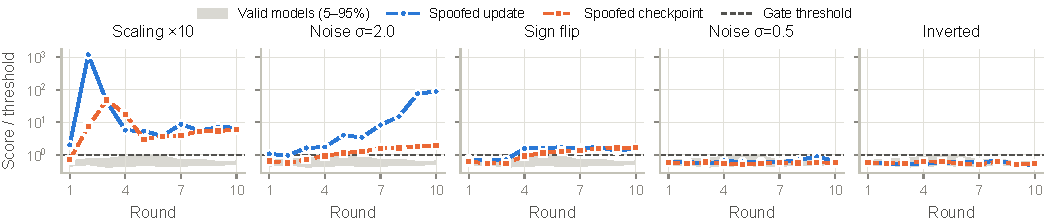
\includegraphics[width=\textwidth]{figures/scores_by_round.pdf}
  \caption{Gate score relative to the per-round threshold (log scale). Grey band: 5--95\% of held-out
  valid models. Lines: median over spoofed models across runs.}
  \label{fig:scores}
\end{figure*}

\begin{figure*}[!t]
  \centering
  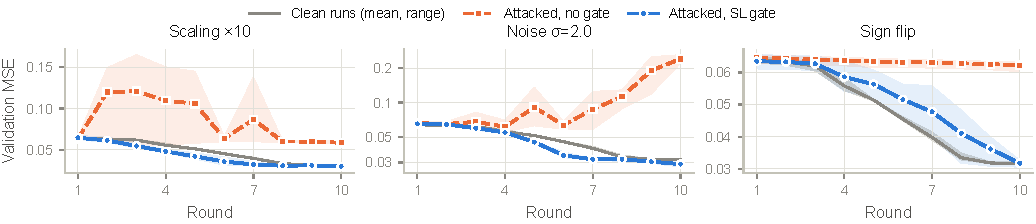
\includegraphics[width=\textwidth]{figures/quality_by_round.pdf}
  \caption{Validation MSE of the global model in force per round: attacked runs without a gate and
  with the final SL gate (mean; shaded: range over runs) against clean runs.}
  \label{fig:quality}
\end{figure*}

\begin{figure*}[!t]
  \centering
  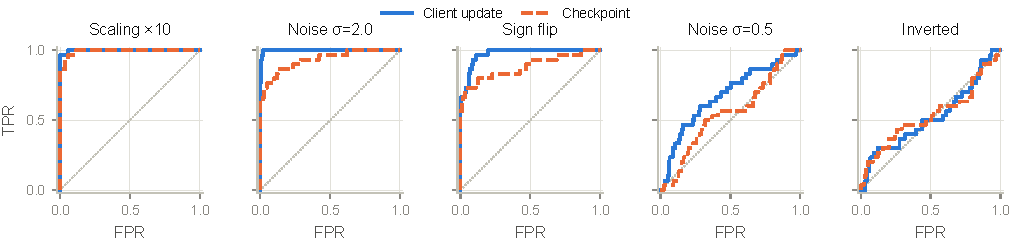
\includegraphics[width=\textwidth]{figures/roc.pdf}
  \caption{ROC of the gate score per attack: spoofed models vs.\ held-out valid models of the same kind.}
  \label{fig:roc}
\end{figure*}

\begin{figure}[!t]
  \centering
  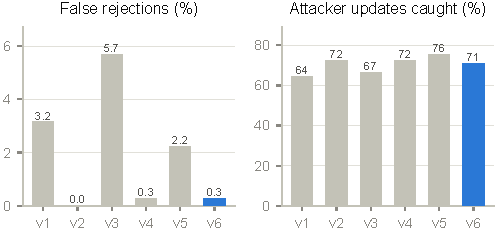
\includegraphics[width=\columnwidth]{figures/versions.pdf}
  \caption{False-rejection rate (honest updates and checkpoints) and attacker detection of each live
  gate version; v6 is the final configuration.}
  \label{fig:versions}
\end{figure}

\begin{figure}[!t]
  \centering
  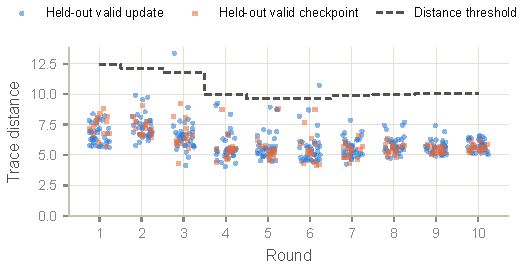
\includegraphics[width=\columnwidth]{figures/calibration.pdf}
  \caption{Leave-one-run-out trace distance of valid models per round and the per-round threshold.}
  \label{fig:calibration}
\end{figure}

\end{document}
